%! TEX root = ../thesis.tex

\chapter{The Pierre Auger Observatory}
\label{chap:auger-observatory}

Located on the argentinian high-plains of Pampa Amarilla, the Pierre Auger observatory is a hybrid detector designed to detect and study cosmic 
rays of the highest energies. With an effective area of \SI{3000}{\kilo\meter\squared} it is by far the largest experiment of its kind 
\cite{DesignReport}.

Altough first proposed in 1992, it took 18 years until the idea of a large scale experiment to detect cosmic rays matured and construction of the 
first prototype started near Mendoza \cite{AugerTimeline}. Some further 20 years later, the Pierre Auger collaboration has co-authored over \TODO
publications and continues to advance research in astroparticle physics.
It does this via a hybrid approach, combining measurements of a surface detector (SD) as well as a flouresence detector (FD). Additional machinery, 
such as the e\textbf{X}treme (XLF) and \textbf{C}entral \textbf{L}aser \textbf{F}acility (CLF), is installed and monitors atmospheric variables. This
improves the overall systematic accuracy of predictions made by the experiment. An overview of the site can be seen in \autoref{fig:auger-array}. Data 
measured by the FD, SD and the atmospheric monitors is sent to a \textbf{C}entral \textbf{D}ata \textbf{A}cquisition \textbf{S}ystem (CDAS) located in 
the nearby town of Malargüe.

This chapter offers a brief look into the measurement principle and setup of the observatory. Information regarding the fluoresence detector can be 
found in \autoref{sec:fluoresence-detector}. The SD is described in \autoref{sec:surface-detector}. A more in depth read on detector specifications 
and design choices is represented by the Pierre Auger observatory design report \cite{DesignReport}, where a lot of information stated in this chapter
is conglomerated from. Notes on the event reconstruction are listed in \autoref{sec:event-reconstruction} and summarized from \cite{SDReconstruction} 
and \cite{FDReconstruction}.

\begin{figure}
	\centering
	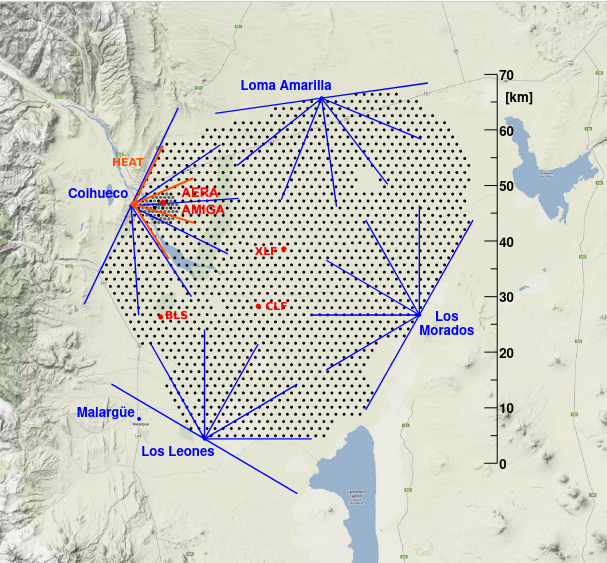
\includegraphics[width=0.9\textwidth]{imgs/auger_array.png}
	\caption{Overview of the Pierre Auger observatory. The four different FD sites (respective FOV shown with blue lines) sit at the edge of
	the detector area and monitor the night sky above the SD array consisting of 1600 water tanks (black dots). A denser spacing of stations 
	near Coihueco is equipped with additional electronics such as e.g. radio antennas (AERA) and muon detectors (AMIGA).}
	\label{fig:auger-array}
\end{figure}

\section{Fluoresence Detector (FD)}
\label{sec:fluoresence-detector}

The FD consists of a total of 27 fluoresence telescopes (eyes) at 4 different sites. Each eye monitors a \SI{30}{\degree} x \SI{30}{\degree} window 
of the sky at a resolution of $\approx \, 0.5 \, \frac{ \text{px} }{ \text{deg}^2 }$. This results in an effective FOV of roughly \SI{180}{\degree} x 
\SI{30}{\degree} per FD station, with an exception of Coihueco, where three additional telescopes - HEAT (\textbf{H}igh \textbf{E}levation 
\textbf{A}uger \textbf{T}elescope) - are installed to enable monitoring of higher zenith angles ($\SI{30}{\degree}\leq\theta\leq\SI{60}{\degree}$) and
increase sensitivity for showers of lower energies (compare \autoref{chap:physical-background}).

The individual telescopes consist of \SI{3.6}{\meter} by \SI{3.6}{\meter}, convex mirrors. They reflect incoming light onto a set of 440 
photomultipliers (PMTs), each corresponding to one pixel in the resulting image seen by an eye. Since the setup needs to be extremely sensitive to 
UV light in order to detect flouresence caused by extensive air showers, its operation is limited to the relatively noise free moonless astronomical 
nights (Sun $\measuredangle$ Horizon $\lesssim-18^{\circ}$). When the FD is operational, this allows the observation of the longitudinal propagation of 
a shower instead of just its' footprint (as seen by the SD). 

\section{Surface Detector (SD)}
\label{sec:surface-detector}

The SD consists of 1600 individually operating stations, spaced apart on a hexagonal grid with a standard \SI{1.5}{\kilo\meter} spacing. Each 
station is made up of a main tank filled with \SI{12000}{\litre} of purified water and reflective inner walls, a solar panel and batteries for power management, 
as well as an antenna for communication. Within each tank three PMTs detect Cherenkov light originating from shower particles, these are together with the tank 
referred to as \textbf{W}ater \textbf{C}herenkov \textbf{D}etectors (WCDs). With the (at the time of this work) ongoing AugerPrime upgrade, each station is 
additionally equipped with a \textbf{S}urface \textbf{S}cintillator \textbf{D}etector (SSD), and radio antenna atop the tank. This allows for finer separation 
of electromagnetic and muonic shower component and detection of highly inclined air showers respectively \cite{AugerPrime, horandel2020precision}. 

Onboard electronics, the \textbf{U}pgraded \textbf{U}nified \textbf{B}oard (UUB), or more precisely six 10-bit \textbf{F}lash 
\textbf{A}nalog-to-\textbf{D}igital-\textbf{C}onverters (FADCs) read out measurement data from the PMTs at a sampling rate of \SI{120}{\mega\hertz} 
($\approx\SI{8.33}{\nano\second}$ binning) \cite{verzi2013energy}. This is done in a two-fold way. Three FADCs digitize the PMTs dynode voltage, resulting in the
\textbf{H}igh\textbf{G}ain (HG) output. Three FADCs monitor the anode voltage to form the \textbf{L}ow \textbf{G}ain (LG) output, which can be analyzed if the 
HG output exceeds a value of $2^{10}$ ADC counts and becomes saturated. This effectively enables the measurement of both large ($\geq\mathcal{O}(10^3)$ particles
hitting the tank) as well as small shower signals ($\mathcal{O}(1)$ particle hitting the tank) with sufficient accuracy. Once an FADC bin has been recorded and 
checked for possible triggers (c.f. \autoref{ssec:sd-triggers}) it is written to a ring buffer. If a trigger is issued, the corresponding chunk in the ring 
buffer (600(? \TODO) bins before and 23409857 bins after the latch bin, where the trigger was raised) can be analyzed in order to calibrate a station in the 
array (\autoref{ssec:sd-calibration}) or processed by a higher-level CPU for event reconstruction purposes (\autoref{sec:event-reconstruction}).

\subsection{Calibration}
\label{ssec:sd-calibration}

While each station is equipped with the same electronics and runs the same analysis software, variables like the position in the field, station age or slight 
changes in the manufacturing/installation process cause different stations to age differently. Over the lifetime of the array such differences can sum into 
potentially drastic discrepancies in gathered data. Put simply, an extensive air shower will look different to a station compared to the same shower one year 
later. To account for this, measurements are standardized for all stations. ADC counts are related to a \textbf{V}ertical \textbf{E}quivalent of through-going
\textbf{M}uons (VEM) that would result in the same signal strength. In this fashion, the maximum response that is generated by a PMT from a vertically 
through-going muon is defined as \SI{1}{\Peak}. The total deposited charge (equivalent to the integral over response) is defined as \SI{1}{\Charge}. The 
conversion factor between ADC counts and VEM$_\text{Peak}$ and VEM$_\text{Ch.}$ is estimated from data and continuously updated via the algorithms detailed 
below. Note that the used methods differ for calibration in the field (Online algorithm) and event reconstruction (Oflline algorithm). Both approaches are listed
here and discussed in more detail in \cite{tobiasBaseline}, \cite{bertou2006calibration}, .

\TODO


\subsubsection{Baseline estimation}
\label{sssec:baseline-estimation}

First and foremost, the average noise level of each PMT needs to be determined

\subsubsection{Rate based estimation of peak and charge}
\label{sssec:online-calibration}


\subsubsection{Histogram based estimation of peak and charge}
\label{sssec:offline-calibration}


\subsection{Trigger procedure}
\label{ssec:sd-triggers}




\section{Event Reconstruction}
\label{sec:event-reconstruction}


